% !TeX root = ../main.tex

\chapter{Introduction}\label{chapter:Introduction}

Sinitic languages as tone languages make use of pitch height and contour to make phonemeic contrasts for lexical tones. For instance, Taiwan Mandarin, one of the Sinitic languages, has four lexical tones: T1, T2, T3, and T4, with T1 being a high-level (55) tone, T2 a mid-rising (35) tone, T3 a low-falling/level (21) tone, and T4 a high-falling (51) tone. In Taiwan Southern Min\footnote{Mainstream Taiwan Southern Min.}, another Sinitic language, there are 7 tones: T1, T2, T3, T4, T5, T7, and T8, with T1 being a high level (55) tone, T2 a high-falling (51) tone, T3 a low level (21) tone, T4 a mid-checked (32) tone, T5 a mid-rising (35) tone, T7 a mid-level (33) tone, and T8 a high-checked (54) tone. While ideally, these tones can be differentiated from each other with their respective pitch values and/or pitch contours, in real-world communication, the actual acoustic realizations of the lexical tones are highly variable, subject to factors including prosody \citep{Peng1997}, syllable duration \citep{XuWang2009}, and tonal coarticulation (\citealp{Shen1990}; \citealp{Xu1994}; \citealp{Peng1997}; \citeyear{Xu1997}; \citealp{Wang2002}; \citealp{ChangHsieh2012}). In this paper, we center into the last factor, i.e., tonal coarticulation, where a target tone's pitch value and/or pitch contour varies owing to preceding and/or following tones, to the extent that it might be acoustically similar to another lexical tone. Specifically, we focus on the perception and production of tonal coarticulation in the two afore-mentioned Sinitic languages: Taiwan Mandarin and Taiwan Southern Min.

%\begin{figure}[hbt!]
%\centering
%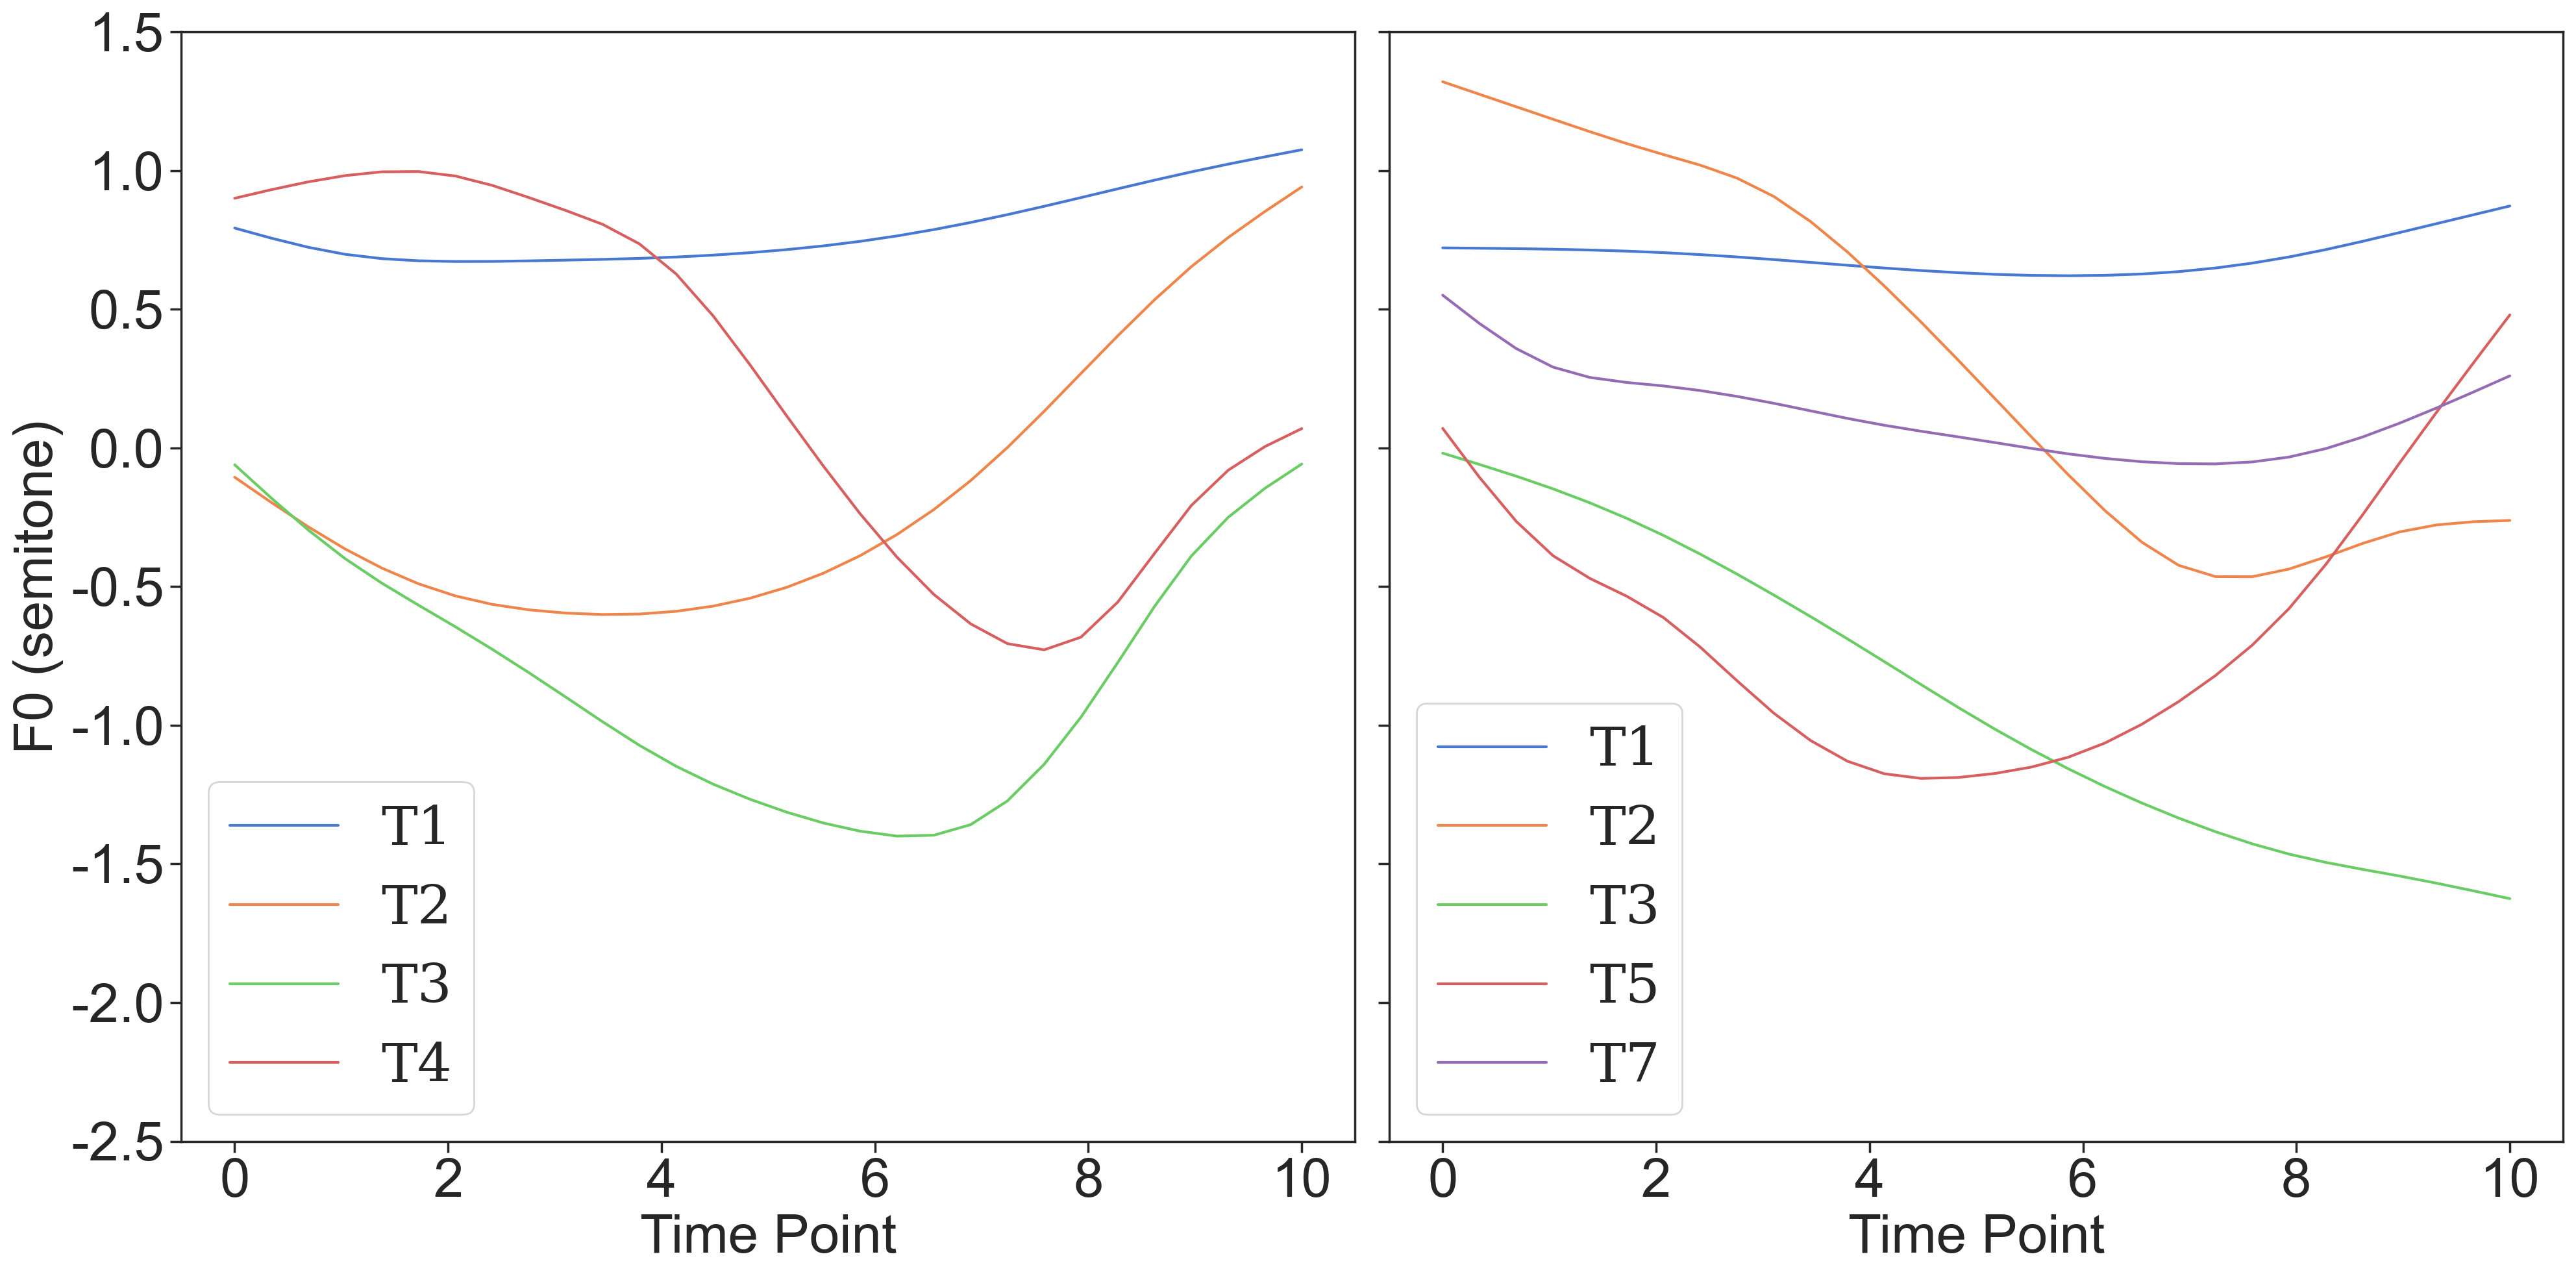
\includegraphics[scale=.3]{Figures/Mandarin_Min_tone_contours.png}
%\caption{Lexical tones in Taiwan Mandarin (left) and Taiwan Southern Min (right)}
%\label{Figure:MandarinMinTones}
%\end{figure}

The variation of one tone under coarticulation with ambient tones was first mentioned in \cite{Chao1968}, where he noted that Mandarin T2 (35) would become T1 when preceded by T1 (55) or T2 (35). While the phonological status of such tonal variation is doubted by some (e.g., \citealp{ShihSproat1992}; \citealp{Xu1994}), follow-up studies generally agree that such variation is acoustically present, and is asymmetric (cf. \citealp{Shen1990}, however, for opposite findings), with carry-over effects (the influence of preceding tones) being stronger and assimilatory, and anticipatory effects (the influence of following tones) being weaker and dissimilatory. A question naturally arises: if the acoustic reality of tones is so fuzzy, how do Mandarin speakers understand them? \cite{Xu1997} investigated this question and found that Beijing Mandarin speakers actually normalized for such tone variation. When a target tone was preceded by a high pitch offset, it was perceived as lower, and vice versa. In this case, a raised T2 (35), which became 55, would still likely be perceived as 35 after normalization.

However, things might be complicated when we turn to Taiwan Southern Min. In Mandarin, there are only 4 tones, and each of them can be distinguished by either tone shape or tone value alone. In Taiwan Southern Min, nevertheless, there are three level tones (T1, T7, T3) that are contrasted only by tone value, and there are 7 tones in total. Intuitively, if the tonal variation is to be as strong as in Mandarin, perception would be much more painstaking. A realized 33 may well be a raised T3 (21), a true T7 (33), or a lowered T1 (55), and a surface T2 (51) may be acoustically very similar to both a raised T3 (21) or T7 (33), and that is only considering carry-over effects. Possible tonal variations in Taiwan Mandarin and Taiwan Southern Min are provided in table \ref{table:Probablevariations}\footnote{The right quotation mark indicates a sandhi tone.}. As we can see, even under tonal coarticulation, the probable allotones in Mandarin still have a general one-to-one relationship, while the same Taiwan Southern Min tones may have multiple correspondences under coarticulatory effects. It is therefore presumable that tonal coarticulation and/or its perception in Taiwan Southern Min might be different from that in Taiwan Mandarin, and the way its speakers deal with such variation may also be different.

\begin{flushleft}
\begin{table}[hbt!]
\begin{tabularx}{\textwidth}{ll|X|X|X|X|}
\hhline{~~----}
 & & T1 (55) & T2 (35) & T3 (21(4)) & T4 (51)\\
\hhline{~~|----}\noalign{\vspace*{\doublerulesep}}
\hhline{--||----}
\multicolumn{1}{|l}{\multirow{2}{*}{Carry-over}} & \multicolumn{1}{l||}{Raised} & - & T1 (55) & T4 (51) & -\\
\multicolumn{1}{|l}{}& \multicolumn{1}{l||}{Lowered} & T2 (35) & - & - & T3 (21)\\
\hhline{--||----}
\multicolumn{1}{|l}{\multirow{2}{*}{Anticipatory}} & \multicolumn{1}{l||}{Raised} & - & - & T2 (35) & T1 (55) \\
\multicolumn{1}{|l}{}& \multicolumn{1}{l||}{Lowered} & T4 (51) & T3 (214) & - & -\\
\hhline{--||----}
\end{tabularx}
\break
\break
\begin{tabularx}{\textwidth}{ll|X|X|X|X|X|}
\hhline{~~-----}
 & & T1/T2' (55) & T2/T3' (51) & T3/T7' (21) & T5 (35) & T7/T1' (33)\\
\hhline{~~|-----}\noalign{\vspace*{\doublerulesep}}
\hhline{--||-----}
\multicolumn{1}{|l}{\multirow{2}{*}{Carry-over}} & \multicolumn{1}{l||}{Raised} & - & - & T7 (33); T2 (51) & T1 (55) & T1 (55); T2 (51)\\
\multicolumn{1}{|l}{}& \multicolumn{1}{l||}{Lowered} & T5 (35); T7 (33) & T7 (33); T3 (21) & - & - & T3 (21)\\
\hhline{--||-----}
\multicolumn{1}{|l}{\multirow{2}{*}{Anticipatory}} & \multicolumn{1}{l||}{Raised} & - & T2' (55) & T1' (33) & - & T2' (55) \\
\multicolumn{1}{|l}{}& \multicolumn{1}{l||}{Lowered} & T1' (33); T3' (51) & - & - & T1' (33) & T7' (21)\\
\hhline{--||-----}
\end{tabularx}
\caption{Probable variations of Taiwan Mandarin (top) and Taiwan Southern Min (bottom) lexical tones under types of coarticulation}
\label{table:Probablevariations}
\end{table}
\end{flushleft}

Indeed, past studies in (Taiwan) Southern Min tonal coarticulation yielded rather different results from what we have seen in (Taiwan) Mandarin. While \cite{Peng1997} and \cite{Wang2002} found anticipatory (Peng and Wang) and carry-over (Wang) effects in Taiwan Southern Min, the effects were symmetric and both assimilatory, unlike the asymmetry attested in (Taiwan) Mandarin. Even, \cite{Lin1988} did not find significant coarticulatory effect in Taiwan Southern Min at all. \cite{ChangHsieh2012}, investigating the same issue in Malaysian Hokkien, a dialect of Southern Min, also found rather inconsistent results, where carry-over and anticipatory effects could be both assimilatory and dissimilatory. While the perception of tonal coarticulation may shed light on this issue, past researches on the perception of Taiwan Southern Min tonal coarticulation are rather sparse. To the author's knowledge, only \cite{Peng1997} and \cite{Wang2002} have investigated this issue. In \cite{Peng1997}, it was discovered that Taiwan Southern Min speakers had an above-chance identification rate of identical syllables followed by different tones even when they were truncated from the original words, which was taken as proof that tonal coarticulation was salient enough to be detected in perception. \cite{Wang2002} also found that tone identification rates were influenced when the ambient tones were swapped, though the results were inconsistent.

Overall it is likely tonal coarticulations in Taiwan Mandarin and Taiwan Southern Min are different, and the normalizing mechanisms of the speakers of the two languages to cope with tone variation are also possibly rather different. However, since no study so far have systemetically investigated and compared the tonal coarticulations of two different tone languages, and the experiment designs, materials used, and the goals of past studies were all different, a direct comparison between two languages is difficult. Crucially, past studies of Mandarin on this issue almost exclusively investigated only Beijing Mandarin. While the two mandarins may share certain similarities on this issue, dialectal variations are also reasonably probable. This paper thus aims to compare the production and perceptual normalization of tonal coarticulations in Taiwan Mandarin and Taiwan Southern Min with systematic and quantifiable designs. Crucially, the following questions are asked: 1) Are the effects of tonal coarticulation of the same magnitude in both Taiwan Mandarin and Taiwan Southern Min? 2) If the effects are of different magnitudes in these two languages, how may speakers of these two languages behave differently in the normalization for tonal coarticulation? 3) If the effects are equally strong in both languages, how then, do Taiwan Southern Min users cope with the possible confusions of lexical tones? One stipulation would be that Taiwan Southern Min does not have such strong tonal coarticulation as in Mandarin, and therefore would not need to compensate for such variation to the same extent as in Mandarin. Another possibility would be that while Taiwan Southern Min does have tonal coarticulation, Taiwan Southern Min users have stricter boundaries between the lexical tones, and therefore would not easily accept a raised/lowered tone as other lexical tones. The last scenario would be that both the production of coarticulated tones and their perception are identical in both Mandarin and Taiwan Southern Min, and that Taiwan Southern Min speakers have to additionally result to other means such as lexicons to enable effective communication. These three scenarios are illustrated in Figure \ref{Figure:ThreePossibleScenarios} as routes C, B, and A respectively.
\begin{figure}[hbt!]
\centering
\begin{tikzpicture}
\node [terminator, text width=.2\textwidth] at (5,0) (block1) {Tone production};

\node [terminator, text width=.2\textwidth] at (1,-2) (block2_1) {Strong tonal coarticulation};
\node [terminator, text width=.2\textwidth ] at (9,-2) (block2_2) {Weak tonal coarticulaiton};

\node [terminator, text width=.2\textwidth] at (5,-4-4) (block3) {Phonetic-level perception};

\node[above, rotate=90] at (-2,-2) {\textbf{Speaker}};

\draw [gray, dotted, thick] (-3, -5) -- (11, -5);

\node[above, rotate=90] at (-2, -9.5) {\textbf{Listener}};

\node [terminator, text width=.2\textwidth] at (1,-6-4) (block4_1) {Loose tonal boundaries};
\node [terminator, text width=.2\textwidth] at (5,-6-4) (block4_2) {Strict tonal boundaries};

\node [terminator, text width=.2\textwidth] at (5,-8-4) (block5) {Phonemic-level perception};

\node [terminator, text width=.2\textwidth] at (5,-10-4) (block6) {Normalization};

\node[draw=none] at (9-.3, -5-4) (text_1) {C};
\node[draw=none] at (1-.3, -5-4) (text_2) {A};
\node[draw=none] at (5-.3, -5-4) (text_3) {B};

\path [connector, color={rgb,255: red, 76; green, 0; blue, 153}] (block1) -| (block2_1);
\path [connector, color={rgb,255: red, 76; green, 153; blue, 0}] (block1) -| (block2_2);

\path [connector, color={rgb,255: red, 76; green, 0; blue, 153}] (block2_1) -- (block3);
\path [connector, color={rgb,255: red, 76; green, 153; blue, 0}] (block2_2) -- (block3);

\path [connector, color={rgb,255: red, 204; green, 0; blue, 0}] (block3) -| (block4_1);
\path [connector, color={rgb,255: red, 0; green, 128; blue, 255}] (block3) -- (block4_2);
\path [connector, color={rgb,255: red, 76; green, 153; blue, 0}] (block3.east) -- (9, -4-4)|-(block5);


\path [connector, color={rgb,255: red, 204; green, 0; blue, 0}] (block4_1) |- (block5);
\path [connector, color={rgb,255: red, 0; green, 128; blue, 255}] (block4_2) -- (block5);

\path [connector, color={rgb,255: red, 204; green, 0; blue, 0}] (block5) -- (block6);

\end{tikzpicture}
\caption{Three possible scenarios of tone perception under tonal coarticulation}
\label{Figure:ThreePossibleScenarios}
\end{figure}
Among the three, routes B and C are not likely to lead to normalization, as the lexical tones are not perceived phonemically as other tones to start with, and therefore no compensation is in need. In route A, additional normalization will be likely since coarticulatorily -raised/-lowered tones are phonmeically recognized as other tones, and listeners may make correction based on the acknowledgement of such variation. Such a route, however, might be less probable in languages with larger inventories of lexical tones, since speakers may not know to what extent they should make the compensation. In Mandarin, a phonetically-realized high falling tone can be reasonably normalized back as a raised 21, while in Southern Min, the options can be both a raised 21 or a distorted 33. While Mandarin listeners need only know that the tone is raise, Southern Min listeners not only have to know that it is raised, but also how much, in order to facilitate faithful normalization. Simply put, the recoverability of the tones is less lower in these languages (cf. \citealp{Flemming2011}).

In the next chapter, we shall first take a more detailed look at tonal coarticulation in (Taiwan) Mandarin and (Taiwan) Southern Min. We then review how tonal coarticulation is perceived in these two languages. In chapter 3, we talk about the experiment designs, data processing and analyses, and test results.
